\documentclass[../main.tex]{subfiles}
\graphicspath{{\subfix{../images/}}}
\begin{document}
\subsection{Well being is a Process of Choice}\index{posture}

We try out movements and wonder: does that {work better}?
Is this movement more fluent?
This process can lead to problems while being in a state of fear, pain or stress.
We then choose the movements we know and bring us relief.

Paradoxically we subconsciously choose \emph{stiff and tensed up movements}.
We don't swing the hips any more, choose confining movements, contract belly and chest and hold the head and neck in a rigid position.
Choosing such habits, a lot of people choose to  {invite difficulties} into their lives.

{Well--being} is therefore a question of knowledge, attitude, our actions and our joy of life.
Our movements influence our whole life.

\subsection{Bad Posture (Load Posture) as Permanent Stress}

\noindent
\begin{minipage}{\textwidth}
\begin{tabular}{p{4cm}p{7.6cm}}

  \raisebox{-0.8\totalheight}{  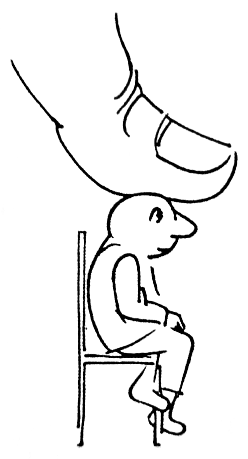
\includegraphics[width=2cm]{Thumb_head} }

  &
The bad posture\footnote{The figures are from~\cite{Haltung} and~\cite{Darmreinig}}\index{posture!bad}, an out--of--alignment posture, is regarded as the {most basic afferent} (from the outside to the brain) impulse for many afflictions of many people. 

Given that the posture influences the psyche of a human being, a physiological posture is important to {center the mind}.\index{posture!psyche} 
\end{tabular}

\noindent
\begin{tabular}{p{7.6cm}p{4cm}}
A good posture only needs a {minimal muscle effort to move} the body with ease.\index{posture!good, natural}
That means that with a good posture no real muscle effort is necessary, because the parts of the skeleton are {balanced} and as close as possible from the {central axis}. 

In the ideal posture, there's exactly the {same tension} on the outer (movement related) muscles and the inner muscles.
{Beside the shape of the spine, the mental sate, the state of the musculature and the physical constitution should be considered for an evaluation of the posture.}
  &
     \raisebox{-0.85\totalheight}{  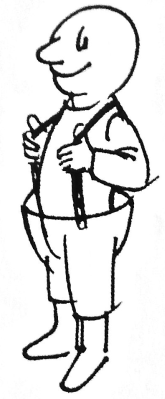
\includegraphics[width=2cm]{Smiling_Guy} }
\end{tabular}
\end{minipage}

\subsection{The physiological posture}\index{posture!physiological}

Which posture is needed to avoid the strain on the structures of the body, which act as disturbances?
The main tell tale sign of a good and natural posture is an {even lordosis} (concave curvature) of the spine between central thoracic spine and the sacrum.
Generally, the term hollow back is understood to refer to the lumbar lordosis, some believe this lordosis to be dangerous.\index{lordosis!lumbar}

The lumbar lordosis (hollow--back) is harmful, if it isn't {pulled up to the middle of the thoracic spine}.
In this position, the spine can carry the body.
The lumbar bone connects in a harmonious arc with the fifth thoracic vertebra between the shoulder blades to carry out its structural function.

\epigraph{Some people carry a hollow back instead of a cross}{translated from \textit{Bert Hellinger}}

Sit on the {front third of the seat}, {open your legs} to about the width of your body. \label{Posture:Sitting}
The soles of both your feet have {contact with the body}.
The point of your toes and your knees point slightly out. 
Your {calves and thighs} have a {right (90\degree) angle} with each other. 

Give a slight {pressure} with the knuckles of your ischium {down} onto the surface of the seat and imagine how the {chair pushes upwards} with the same force upwards.
That will automatically make you hold your upper body in an upright position.

        \begin{figure}[htb!]
          \centering
          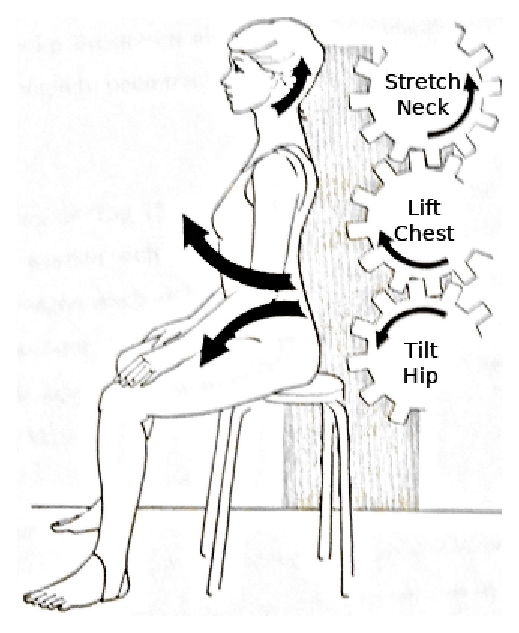
\includegraphics[width=6cm]{phys_posture}
           \caption{Physiological posture in seated position~\cite{Haltung}}
        \end{figure}

This is the {normal posture}, where the chest and the belly cavity give the inner {organs enough space} and in which the {spine} can fulfill its carrying function and act as the {central axis}. 
When the body gets straightened up while seating, it will automatically {tilt the hip forward}, the {chest gets lifted} and the {cervical spine stretched}.
At the same time, the shoulder girdle will be placed in the right place.
The opposite is also true: if somebody lets themselves fall into a {bend posture}, the {chest sinks}, the {hip rolls back} and the {shoulder girdle moves forward}. That makes the {cervical spine} have a {concave curvature}.

\subsection[The Bad Posture and It's Effects]{The Bad (Out--of--Alignment) Posture and It's Effects}\index{posture!bad}

It's not only the {skeleton} which experiences a strain in a bad posture, also the {visceral cavity} gets affected negatively.
The {pressure} which we seemingly are exposed to, puts pressure on our \emph{psyche} and mood.

The strain of the bad posture leads to a {mechanical strain} of the {musculoskeletal system}.
This strain significantly {reduces the mechanical load capacity}.
On the other side, this leads our body to react with {protective measures} to counteract that strain.

Only the physiological posture grants {optimal spatial conditions} in the visceral cavity.
Every curvature of the spine {contracts the organs} of the chest and the belly region.
A {physical evasion} is possible, but severely {impairs the function} of the organs.

Think about it that way: every single human makes between {15,000 and 30,000 breaths every day}.
Over weeks and months, even the smallest {errors accumulate} and will lead to tangible consequences.
A bad posture with {tense abdominal muscles} and {inhibited diaphragm} or then {caved in shoulders} with {constricted visceral cavity}
(often all of that) will inhibit up to 30,000 times daily the breath.

In a bad posture, our {vestibular} comes into a {zone of depression}.
A physiological posture is necessary for an optimal state of the psyche. 
A bad posture leads to {unnecessary tension and pressure} in our body, which in turn leads to our body constantly being in a {fight}.
This will affect our {thinking patterns}.
Fight never leads to peace.
Without peace, our progress will be stunted.

\newpage
\subsection{Compare and Contrast}

\begin{minipage}{\textwidth}
\begin{tabular}{p{6.3cm}p{6.3cm}}
  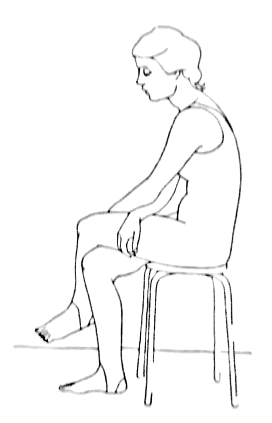
\includegraphics[width=4cm]{Sitting_posture_Bad} &

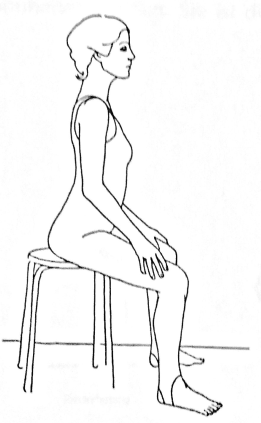
\includegraphics[width=4cm]{Sitting_posture_Good} \\

  \begin{enumerate}
\item {Sunken chest}\footnote{The pictures are from~\cite{Haltung} and~\cite{Darmreinig}}
\item Hip erect
\item Kyphosis\footnote{Kyphosis: backwards curvature of the spine} with a big {curvature} of the lumbar, thoracic and lower cervical {spine}
\item Compensatory lordosis\footnote{Lordosis: forward curvature of the spine}
  of the central cervical spine
\item Reclination\footnote{Reclination: Backwards bending of the neck}
  of the upper cervical spine (``head joint'')
\item {Forward falling of the shoulders}
\item Non--physiological leg and feet axes
    \end{enumerate} &

  \begin{enumerate}
\item {Chest lifted}
\item Hip tilted
\item Harmonic thorax--columbal (chest--loin) {lordosis} from the fifth thoracic vertebra to the sacrum.
\item Cervical spine (neck) stretched
\item Cranio--cervical inclination\footnote{Inclination: Forward bending of the head} ({chin to larynx})
\item Retro position\footnote{Retro position: Backwards shift} of the shoulders ({shoulder girdle rests on the thorax})
\item Physiological leg and feet axes

    \end{enumerate}
\\
  
  \end{tabular}
\end{minipage}

\newpage
\subsection{Habitual Behaviors Determine our Posture}

Our posture is influenced by our habitual behaviors and is the outward expression of our feelings.
\begin{figure}[h!]
  \centering
  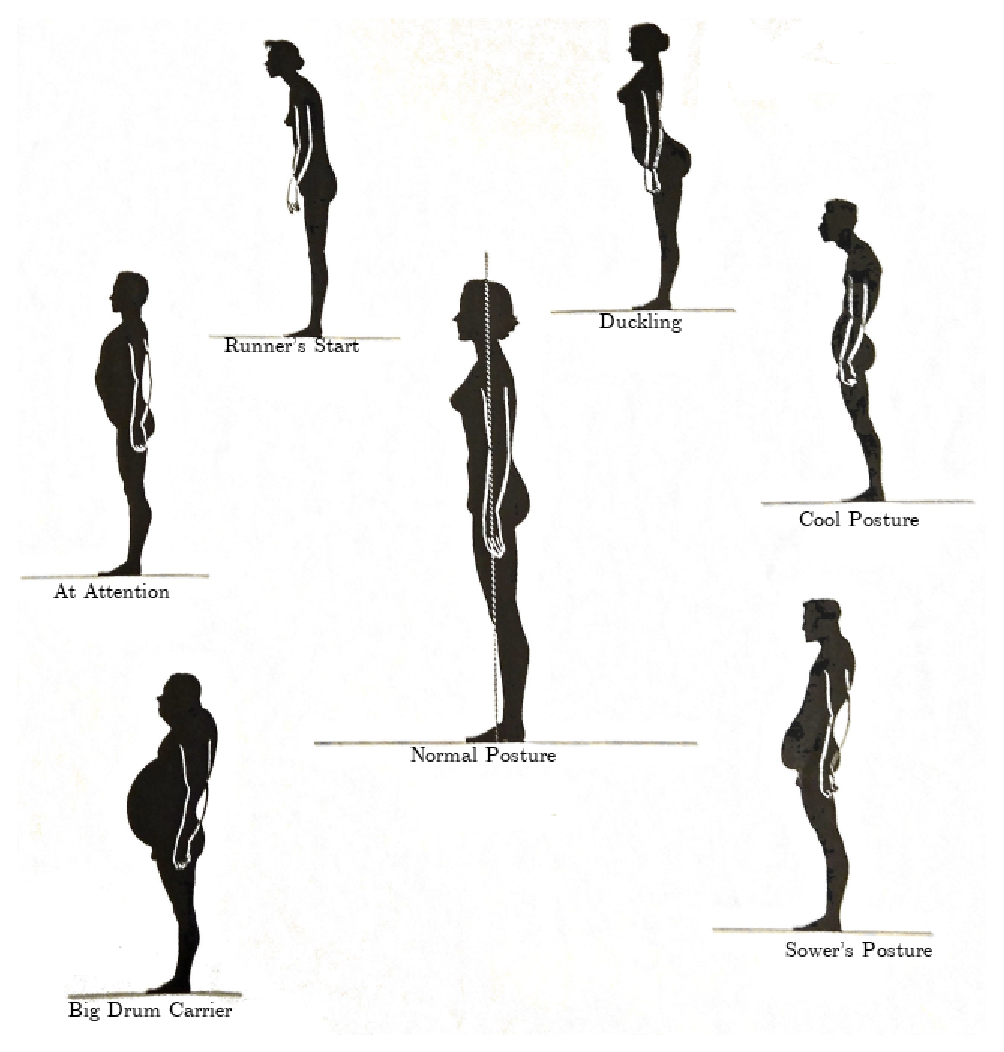
\includegraphics[width=13cm]{Wrong_Postures}
  \caption{Postures in standing position~\cite{Haltung}}
\end{figure}
\newpage

\subsection{Permanent Stress in the Brain}

\begin{figure}[h!]
  \centering
  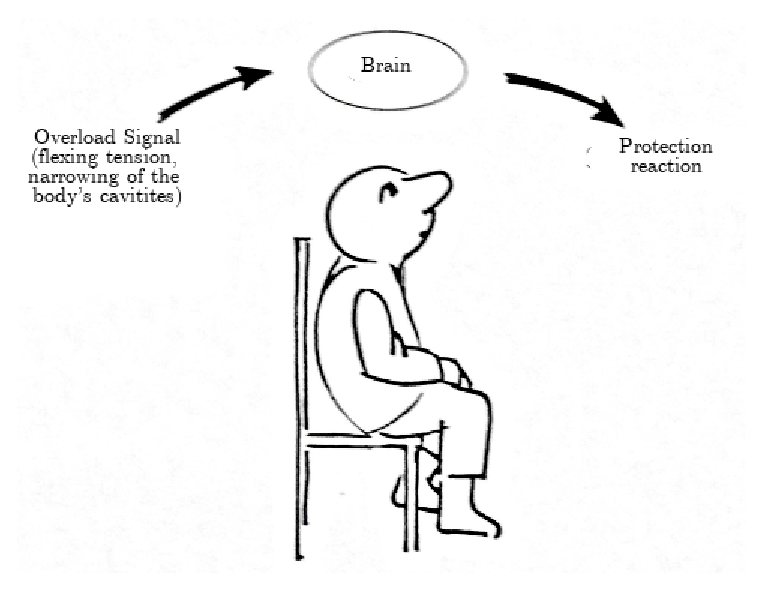
\includegraphics[width=11cm]{Sitting_guy}
  \caption{Bad posture causing permanent stress.~\cite{Haltung}}
\end{figure}

The straining, bad posture has to be overcome, because otherwise it will constantly send signals of being overtaxed which will in turn cause protection mechanisms in our bodies.
These protection mechanisms avoid us from correcting our posture back to normal, what means nothing else but permanent stress.

\epigraph{You shall do something good for your body, so that your soul feels like living in it.}{\textit{Winston Churchill}}
  
\end{document}